\documentclass[a4paper,12pt]{report} 
\usepackage[utf8x]{inputenc}
\usepackage[french]{babel}
\usepackage{mathtools}
\usepackage{amsmath}
\usepackage{amsfonts}
\usepackage{amssymb}
\usepackage{textcomp}
\usepackage[nointegrals]{wasysym}			% Collection de symboles mathématiques
\usepackage{multicol}					% Pour utiliser \hfill
\usepackage{ifthen}
\usepackage{tabularx}	 				% Gestion avancée des tableaux
%\usepackage{cleveref}

\usepackage{float}

\usepackage{enumitem}
\usepackage{wrapfig}
%\usepackage[squaren]{SIunits}
%\usepackage[T1]{fontenc}				% Indispendable, présent dans tous les codes exemples
\usepackage[linkcolor=DarkGreen,colorlinks=true, citecolor= DarkGreen, urlcolor=MidnightBlue]{hyperref} 	% Hyper ref
\usepackage{listings}					% Pour citer du code
\usepackage[justification=centering]{caption}
\usepackage{sistyle} 
\usepackage{numprint}
\usepackage{wrapfig}
\usepackage{cite}	
\usepackage{url} 					% Pour citer les sites internet dans la
%\usepackage{cleveref}
\usepackage{setspace}

\usepackage{graphicx}		 			% Inclusion des figures
\graphicspath{{./pic/}, {./../figures/ML}}
\usepackage[svgnames]{xcolor}			%https://www.latextemplates.com/svgnames-colors

%%% Commandes utiles définies
\newcommand{\argmin}{\mathop{\mathrm{argmin}}}

\newcommand{\bepar}[1]{
	\left( #1 \right)  
}

\newcommand{\becro}[1]{
	\left[ #1 \right]  
}

\newcommand{\rbk}[1]{\color{red}\textit{#1} \color{black}  
}

\usepackage{listings}					% Pour citer du code
%%%%%%%%%%%%%%%%%%%
%%% Élément pour citer des codes %%%
\lstset{
language=Python,
basicstyle=\ttfamily\bfseries\small, %
identifierstyle=\bfseries\color{black}, %
keywordstyle=\color{blue}, %
stringstyle=\color{black!90}, %
commentstyle=\it\color{black!70}, %
columns=flexible, %
tabsize=4, %
extendedchars=true, %
showspaces=false, %
showstringspaces=false, % %
numberstyle=\small, %
breaklines=true, %
breakautoindent=true, %
captionpos=b,
otherkeywords={cross_val_score},
keywords=[0]{cv},
keywordstyle=[0]{\color{red}},
}
%%%%%%%%%%%%%%%%%%%%%
%\usepackage{multicol}
%\usepackage{etoolbox}
%\patchcmd{\thebibliography}{\section*{\refname}}
%    {\begin{multicols}{2}[\section*{\refname}]}{}{}
%\patchcmd{\endthebibliography}{\endlist}{\endlist\end{multicols}}{}{}
\usepackage[authoryear]{natbib}

\usepackage{geometry}
\geometry{hmargin=2cm, vmargin=2cm}

%%%%%%%%%%%%%%%%%%%%
%%% Couleurs %%%
\xdefinecolor{brick}{named}{DarkRed}
\xdefinecolor{navy}{named}{Navy}
\xdefinecolor{midblue}{named}{MidnightBlue}
\xdefinecolor{dsb}{named}{DarkSlateGray}
\xdefinecolor{dgreen}{named}{DarkGreen}

%%% 	Raccourcis 	%%%
\newcommand{\keps}{$k-\varepsilon$}
\newcommand\bk{\color{black}}
\newcommand\brick{\color{brick}}
\newcommand\navy{\color{navy}}
\newcommand\midblue{\color{midblue}}
\newcommand\dsb{\color{dsb}}
\newcommand{\dgreen}{\color{dgreen}}
\newcommand\red{\color{red}}

%%%%%%%% Cigles
\newcommand{\rap}{par rapport}
\newcommand{\cad}{c'est-à-dire}
\newcommand{\vav}{vis-à-vis}

%%%%%%%% Autres

%% Columns
\usepackage{multicol}		% Pour utiliser \hfill et découper une partie de son texte en colonnes
\setlength{\columnseprule}{0.pt}
%\def\columnseprulecolor{\color{red}}
%\setlength{\columnsep}{1.5cm}

%%%%%%%%%%%%%%%%%%%
% Syntax: \colorboxed[<color model>]{<color specification>}{<math formula>}
\newcommand*{\colorboxed}{}
\def\colorboxed#1#{%
  \colorboxedAux{#1}%
}
\newcommand*{\colorboxedAux}[3]{%
  % #1: optional argument for color model
  % #2: color specification
  % #3: formula
  \begingroup
    \colorlet{cb@saved}{.}%
    \color#1{#2}%
    \boxed{%
      \color{cb@saved}%
      #3%
    }%
  \endgroup
}
\title{\navy \textbf{Notes Machine Learning} \color{black}}%%%%%%%%%%%%%%%%%%%%
\date{}

\renewcommand{\sectionmark}[1]{\markright{#1}}
\usepackage{fancyhdr}
\pagestyle{fancy}
\lhead{\textbf{Nathaniel} \brick \textbf{\textsc{Saura}}}
\rhead{\markright}
\cfoot{\thepage}
\renewcommand{\headrulewidth}{0.4pt}

\numberwithin{equation}{section} %%%% To count the equation like Section.Number

\begin{document}
\maketitle
\chapter{Présentation}
Réseaux de neurones : ensemble d'opération mathématiques visant à ajuster les hyperparamètres du réseaux pour associer la meilleure sortie à une entrée donnée. \\
Deux phases : une phase d'entraînement pour laquelle les entrées et les sorties sont fournies à l'algorithme et une phase de prédiction ou seule les entrées sont fournies.\\
Pendant la phase d'entraînement les poids et biais (hyperparamètres) liant chacune des couches cachées entre elles, sont ajustés de sorte à minimiser l'erreur commise entre la prédiction et la sortie espérée, à chaque époque.\\

\noindent The equation we focus on is the Viscous Burgers Equation (VBE):
\begin{equation*}
\frac{\partial u}{\partial t} + u \frac{\partial u}{\partial x} = \nu \frac{\partial^2 u}{\partial x^2} 
\end{equation*}

We want to estimate if it's possible to predict the velocity field at each temporal iteration using a neural network (NN). In a mathematical formulation, we want to obtain  
\begin{equation*}
u^{n+1} = \mathcal{F}\bepar{u^n}	
\end{equation*}
Where $\mathcal{F}$ is a function whose arguments come from the current velocity field (n-th iteration).\\
In this report we evaluate 3 different architectures and 3 different number of features i.e. 3 different number of columns in the matrix $X$.\\
We will also present the bootstraping method and its results with the three architectures and for each number of features choosen.

\pagebreak

\section*{Architecture N3}
\noindent Whichever considered architecture, the dataset is constructed with the resolution of each of the initial condition displayed in Fig.\eqref{ci}. We use the Lax-Wendroff scheme to solve this problem with periodic boundary conditions.\\
We choose to focus on the first 60 iterations (itmax in the following), that marks the apparition of the choc and its flaring.\\
We'll see for each case how we built the $X$ and $y$ matrices, the data and its target respectively. \\
We do not seek to adjust hyperparameter of the NN but we will consider two different activation function : "MSEGrad" presented in the last Duraisamy paper and the classical "Lasso". We use TensorFlow library, Adam optimizer and a learning rate constant to 0.001.\\
The subscript $_j$ refers to the $j$-th point of the problem spatial discretization : $j \in \ \{ 0, N_x-1 \}$.\\
The superscript $^n$ refers to the $n$-th iteration of the problem temporal discretization : $n \in \{ 0, N_t-1 \}$. \\
At the end, the resp. dimensions of $X$ and $y$ are : 
$$\dim\left(X \right) = \left(n_{\text{init}} \times (N_x - 2) \times (\text{itmax} - 1),\ n_{\text{features}}\right) $$
$$ \dim \left(y \right) = \left(n_{\text{init}} \times (N_x - 2) \times (\text{itmax} - 1), \ 1 \right) $$

\begin{figure}[!ht]
\centering
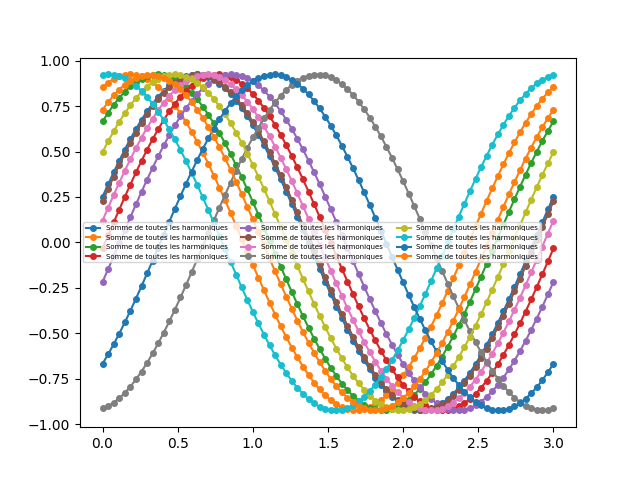
\includegraphics[scale=1]{/CI.png}
\caption{Conditions initiales de cas pour la construction du train set. Toutes ces situations sont résolues à partir d'un solver Lax-Wendroff pour 60 itérations. Les champs de vitesses pour toutes les itérations sont agglomérés dans une matrice $X$ la cible correspondante est enregistrée dans une matrice $y$}
\label{ci}
\end{figure}

\pagebreak

\section*{Architecture N5, epoch 200}
\subsection*{Stencil with the derivative}
We build $X$ and $y$ as : 
\begin{multicols}{2}
\begin{equation*}
X = 
\left[ 
	\begin{array}{c} 
		\dots \\
		\dots \\
		u_{j-1}^n,\ u_j^n,\ u_{j+1}^n, \frac{u_{j+1}^n - u_{j-1}^n}{2 \Delta x} \\
		\dots \\
		\dots  
	   \end{array}
\right]
\end{equation*}

\columnbreak

\begin{equation*}
y = 
\left[ 
	\begin{array}{c}
		\dots\\
		\dots\\
		u_{j}^{n+1} \\
		\dots\\
		\dots
	\end{array}
\right]
\end{equation*}
\end{multicols}

\noindent Here $n_{\text{features}} = 4$, we use a centered stencil around $j$ along with the centered derivative around $u_j^n$. Nothing more to say on $y$.\\

An important variable to consider will be 
\begin{equation}
  U^{n+1}_{\text{MLpred}} - U^{n+1}_{\text{exact}} \tag{\navy Relative error\bk} \label{r_error}
\end{equation}  
We test on 3 different initial conditions. The three different figures shown below are screenshots after 55 iterations. \\
The upper-left graph sketches the \ref{r_error} between the predicted and the exact velocity field in the whole domain. The upper-right graph sketches the evolution of the infinite norm of the \ref{r_error} through the temporal iteration. Final the lower graph sketches the plot of the exact solution and the prediction.\\

\begin{figure}[H]
\centering
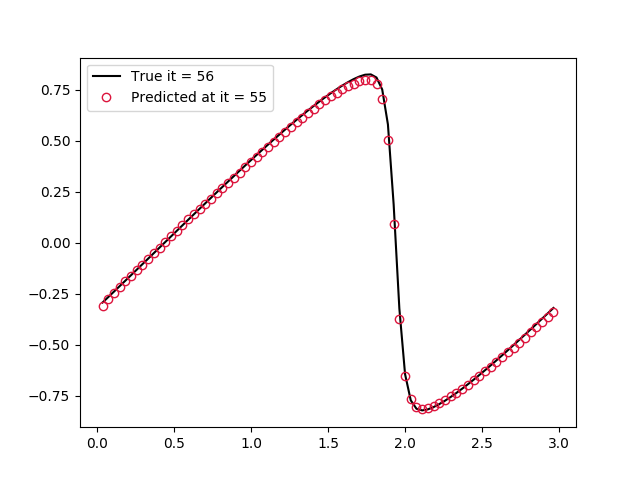
\includegraphics[scale=0.5]{/itmax_60_N5_epoch200/NN_solution_DER_case.png}
\caption{}
\label{derN5_200_c1}
\end{figure}

\begin{figure}[H]
\centering
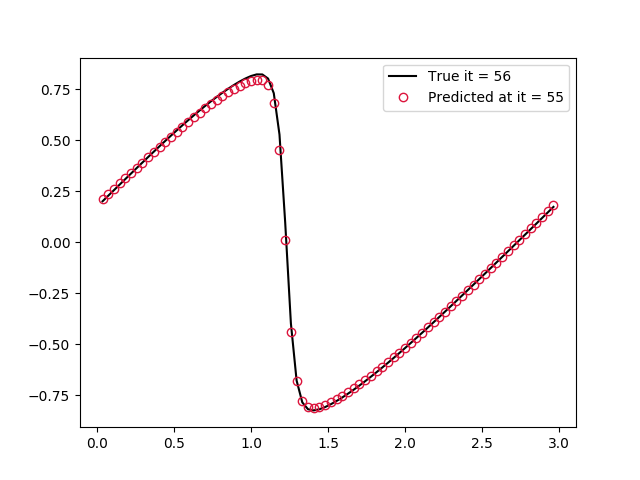
\includegraphics[scale=0.65]{/itmax_60_N5_epoch200/NN_solution_DER_case_2.png}
\caption{}
\label{derN5_200_c2}
\end{figure}

\begin{figure}[H]
\centering
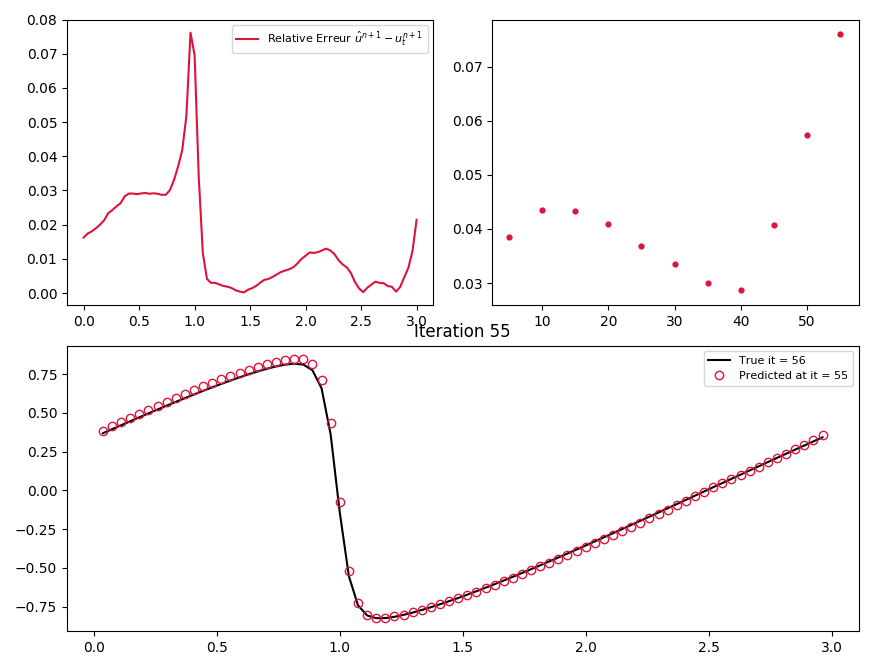
\includegraphics[scale=0.65]{/itmax_60_N5_epoch200/NN_solution_DER_case_3.png}
\caption{}
\label{derN5_200_c3}
\end{figure}

\pagebreak

\subsubsection*{Use of bootstrap}
\noindent Now we use the bootstrap method to try to build a more robust model. The bootstrap idea is to sample several times the initial dataset, and train a NN on each sample. \\
The prediction is then the mean of all the NN predictions and we can even have access to the the variance. Here we choosed 5 estimators (5 samples, so 5 NN) and we sketch three graphs with the same structure detailed above :

\begin{figure}[H]
\centering
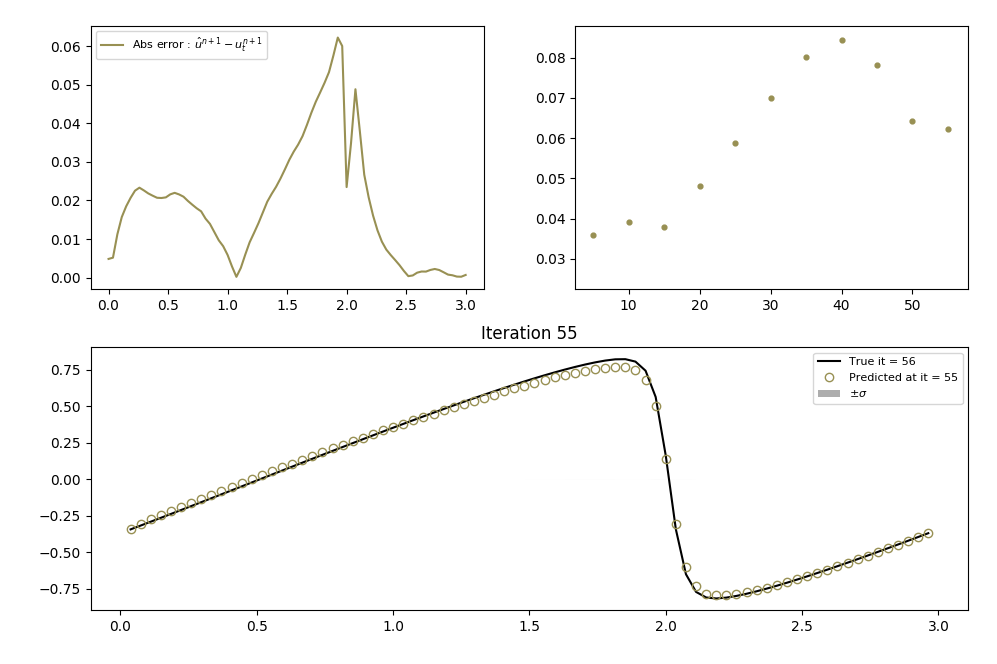
\includegraphics[scale=0.65]{/itmax_60_N5_epoch200/Boot_solution_DER_case.png}
\label{bootderN5_200_c1}
\end{figure}

\begin{figure}[H]
\centering
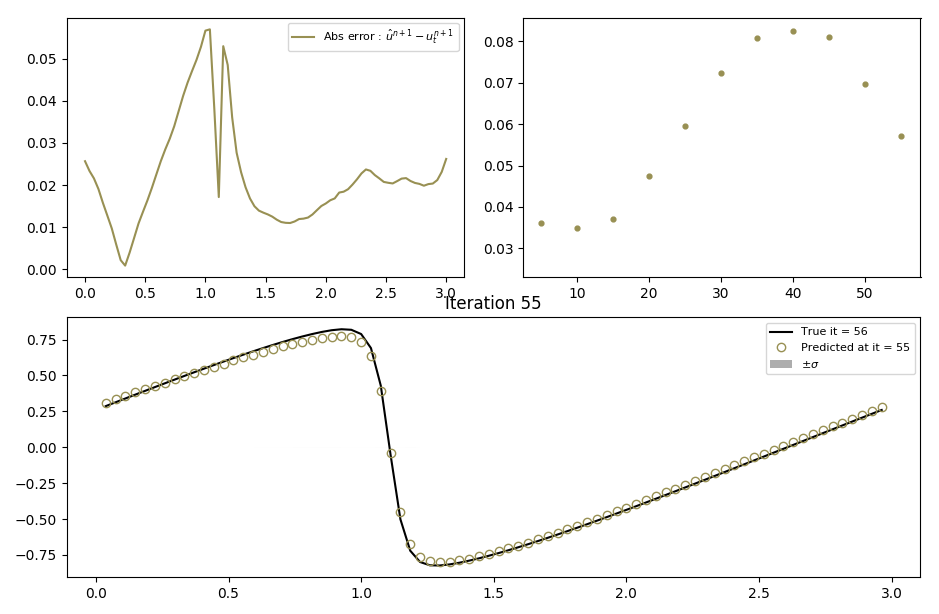
\includegraphics[scale=0.6]{/itmax_60_N5_epoch200/Boot_solution_DER_case_3.png}
\label{booderN5_200_c3}
\end{figure}

\begin{figure}[H]
\centering
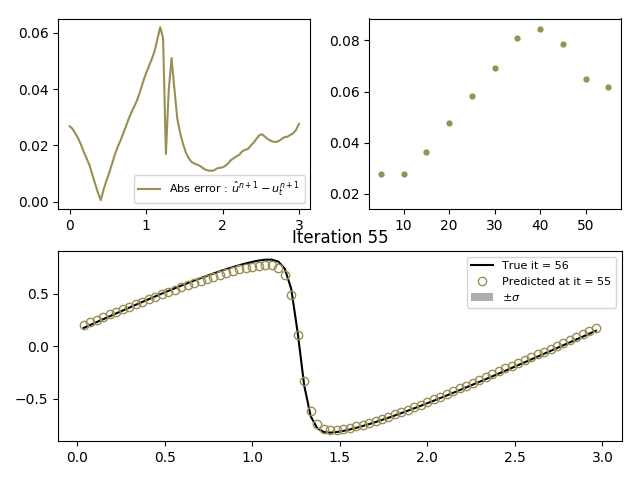
\includegraphics[scale=0.8]{/itmax_60_N5_epoch200/Boot_solution_DER_case_2.png}
\caption{}
\label{bootderN5_200_c2}
\end{figure}





\end{document}